\section{BÀI TẬP CUỐI CHƯƠNG 5}
\subsection{Câu hỏi trắc nghiệm}

\Opensolutionfile{ans}[ans/ans-9C5-OTC]
\begin{ex}%[Dự án EX-9-Đề Cương Toán 9]%[Phạm Hoàng Điệp]%[9H5H1]
Trong mặt phẳng tọa độ $Oxy$, cho các điểm $A(3;0)$, $B(-2;0)$ và đường tròn $(C)$ tâm $O$, bán kính bằng $3$. Khi đó vị trí tương đối của các điểm $A$ và $B$ với đường tròn $(C)$ là
\choice
{Điểm $A$ và $B$ nằm ngoài đường tròn $(C)$}
{Điểm $A$ và $B$ nằm trên đường tròn $(C)$}
{Điểm $A$ nằm ngoài đường tròn $(C)$ và điểm $B$ nằm trên đường tròn $(C)$}
{\True Điểm $A$ nằm trên đường tròn $(C)$ và điểm $B$ nằm trong đường tròn $(C)$}
\loigiai{
\immini{
Dựa vào hình vẽ ta thấy
\begin{itemize}
\item Điểm $A$ nằm trên đường tròn $(O;3)$.
\item Điểm $B$ nằm trong đường tròn $(O;3)$.
\end{itemize}
}{
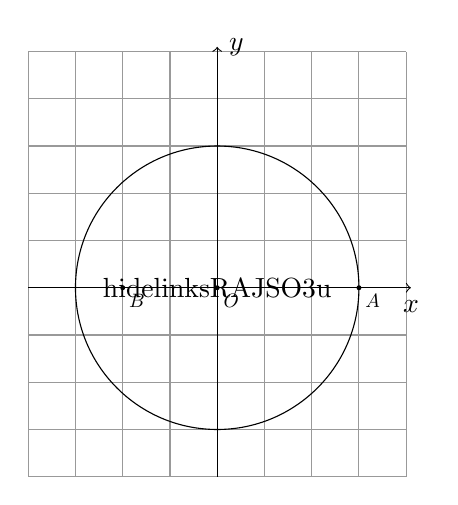
\begin{tikzpicture}[scale=0.6,every node/.style={minimum size=0.5cm-\pgflinewidth, outer sep=0pt}]
\draw[step=1cm,color=black!40] (-4,-4) grid (4,5);
\draw[->] (-4,0)--(4.1,0) node[below] {$x$};
\draw[->] (0,-4)--(0,5.1) node[right] {$y$};
\coordinate (tam) at (0,0);
\coordinate (B) at (-2,0);
\coordinate (A) at (3,0);
\def\bankinh{3}
\draw (tam) circle [radius=\bankinh];
\fill (tam) circle[radius=1.5pt] node[scale=0.7,below right] {$O$}
(B) circle[radius=1.5pt] node[scale=0.7,below right] {$B$}
(A) circle[radius=1.5pt] node[scale=0.7,below right] {$A$}
;
\path (0,0) node{\hypersetup{hidelinks}\href{RAJSO3u}{ }};
\end{tikzpicture}
}
}
\end{ex}



\begin{ex}%[Dự án EX-9-Đề Cương Toán 9]%[Phạm Hoàng Điệp]%[9H5H2]
\immini{Tâm $O$ của một đường tròn cách dây $AB$ của nó một khoảng $3$ cm. Dây $AB$ dài $8$ cm. Khi đó bán kính là
\choice
{\True $5$ cm}
{$4$ cm}
{$6$ cm}
{$3$ cm}}
{
\begin{tikzpicture}[declare function={r=1.8;ga=-150;gb=-30;},font=\scriptsize]
\path (0,0) coordinate (O) %tam
(ga:r) coordinate (A)
(gb:r) coordinate (B)
($(A)!(O)!(B)$) coordinate (H);
\draw (O) circle (r) (A)--(O)--(B)--cycle (O)--(H);
\foreach \t/\g in {A/180,B/0,O/90,H/-90}{
\fill (\t) circle (1pt) node[shift={(\g:7pt)}]{$ \t $};		}
\path pic[draw,angle radius=5pt]{right angle= A--H--O};
\end{tikzpicture}
}
\loigiai{
Kẻ $OH$ vuông góc với $AB$ tại $H$, khi đó $H$ là trung điểm $AB$ hay $AH = \dfrac{AB}{2}=\dfrac{8}{2}=4$ cm.\\
Tam giác $AHO$ vuông tại $O$. Áp dụng định lý Pythagoras: $R = \sqrt{4^2 + 3^2} = \sqrt{25} = 5$ cm.
}
\end{ex}



\begin{ex}%[Dự án EX-9-Đề Cương Toán 9]%[Phạm Hoàng Điệp]%[9H5H2]
Góc ở tâm chắn cung $120^\circ$ có số đo là
\choice
{$60^\circ$}
{\True $120^\circ$}
{$90^\circ$}
{$30^\circ$}
\loigiai{
Góc ở tâm chắn cung $120^\circ$ có số đo bằng $120^\circ$.
}
\end{ex}



\begin{ex}%[Dự án EX-9-Đề Cương Toán 9]%[Phạm Hoàng Điệp]%[9H5H3]
Một hình quạt có góc ở tâm là $60^\circ$, bán kính $6$ cm. Diện tích hình quạt là
\choice
{$\pi$}
{\True $6\pi$}
{$36\pi$}
{$12\pi$}
\loigiai{
Diên tích hình quạt là	$S = \frac{60}{360} \cdot \pi \cdot 6^2 = \frac{1}{6} \cdot \pi \cdot 36 = 6\pi$ (cm$^2$).
}
\end{ex}

\begin{ex}%[Dự án EX-9-Đề Cương Toán 9]%[Phạm Hoàng Điệp]%[9H5H3]
Độ dài cung $40^{\circ}$ của đường tròn bán kính $9$ cm là
\choice
{\True $2\pi$}
{$\pi$}
{$3\pi$}
{$4\pi$}
\loigiai{
Độ dài cung $40^{\circ}$ của đường tròn bán kính $9$ cm là
\[l=\dfrac{40}{180}\cdot\pi\cdot9=2\pi~\text{(cm)}.\]
}
\end{ex}

\begin{ex}%[Dự án EX-9-Đề Cương Toán 9]%[Phạm Hoàng Điệp]%[9H5H3]
Diện tích của hình vành khuyên nằm giữa hai đường tròn đồng tâm có bán kính là $3$ m và $6$ m là
\choice
{$16\pi$}
{\True $27\pi$}
{$20\pi$}
{$3\pi$}
\loigiai{
Gọi $S_{v}$ là diện tích cần tính.\\
Ta có $S_{v}=\pi\left(6^2-3^2\right)=27 \pi$ (m$^2$).
}
\end{ex}


\begin{ex}%[Dự án EX-9-Đề Cương Toán 9]%[Phạm Hoàng Điệp]%[9H5H5]
Cho hai điểm $O$ và $O'$ sao cho $OO'=5$ cm. Vị trí tương đối giữa hai đường tròn $\left(O;4 \,\text{cm}  \right)$ và $\left(O';3 \,\text{cm}  \right)$ là
\choice
{\True Cắt nhau}
{Tiếp xúc trong}
{Tiếp xúc ngoài}
{Không giao nhau}
\loigiai{
Ta có $OO'=5$ cm.\\
Đặt $R=4$ cm; $R'=3$ cm, ta thấy $1 \, \text{cm} \, < 5 \, \text{cm} \, < \, 7 \, \text{cm}$, nên 	$R-R'<OO'<R+R'$. Do đó, hai đường tròn đã cho cắt nhau.
}
\end{ex}

\begin{ex}%[Dự án EX-9-Đề Cương Toán 9]%[Phạm Hoàng Điệp]%[9H5H2]
\immini{Số đo góc $MIN$ trong hình vẽ bên là
\choice
{$100^\circ$}
{$200^\circ$}
{\True $50^\circ$}
{$30^\circ$}
}
{\begin{tikzpicture}[line join = round, line cap = round,>=stealth,font=\footnotesize,scale=0.7]
\def\r{2}
\path
(0,0) coordinate (O)
(\r,0) coordinate (X)
($(O)!1!-10:(X)$) coordinate (M)
($(O)!1!-120:(X)$) coordinate (N)
($(O)!1!110:(X)$) coordinate (I)
;
\draw (O) circle(\r cm);
\draw (M)--(I)--(N)--(O)--(M);
\foreach \x/\g in {O/90,M/-10,N/-120,I/110}\fill[black] (\x) circle (1pt) ($(\x)+(\g:3mm)$) node{$\x$};
%\draw (0,-2) node[below]{n};
%\draw (-90:2) node[below]{m};
\draw (-55:0.8) node[scale=0.8]{$100^\circ$};
\foreach \a/\b/\c in {N/O/M,N/I/M}{\draw pic[draw,angle radius=3mm] {angle = \a--\b--\c};}
\foreach \a/\b/\c in {N/O/M}{\draw pic[draw,angle radius=3.5mm] {angle = \a--\b--\c};}
\end{tikzpicture}}
\loigiai{Xét đường tròn $(O)$ có
$\widehat{MON}$ là góc ở tâm và $\widehat{MIN}$ là góc nội tiếp cùng chắn cung $MN$ nên
$$
\widehat{MIN}=\dfrac{1}{2}\widehat{MON}=\dfrac{1}{2}\cdot 100^{\circ}=50^{\circ}.
$$
Vậy $\widehat{MIN}=50^{\circ}$.}
\end{ex}



\begin{ex}%[Dự án EX-9-Đề Cương Toán 9]%[Phạm Hoàng Điệp]%[9H5H4]
Cho hai tiếp tuyến $PA$ và $PB$ của đường tròn $(O;R)$ ($A$ và $B$ là hai tiếp điểm), biết $R=2$ cm và $OP=4$ cm. Độ dài $AP$ bằng
\choice
{$2\sqrt{5}$}
{\True $2\sqrt{3}$}
{$2\sqrt{6}$}
{$3\sqrt{3}$}
\loigiai{
\begin{center}
\begin{tikzpicture}[scale=1, font=\footnotesize, line join=round, line cap=round, >=stealth]
\coordinate[label=right:$O$] (O) at (0,0);
\coordinate[label=left:$P$] (C) at (-5,0);
\draw[name path=circleO] (O) circle[radius=2cm];
\path[name path=circleX] let \p1=($(O)-($(O)!.5!(C)$)$) in ($(O)!.5!(C)$) circle ({veclen(\x1,\y1)});
\path[name intersections={of= circleX and circleO}] coordinate (A) at (intersection-1) coordinate (B) at (intersection-2);
\path (intersection of A--B and C--O) coordinate (D) node[below left]{$H$} ;
\draw (C)--(A)node[above]{$A$}--(O)--(B)node[below]{$B$}--(C)--(O) (A)--(B);
\foreach \diem in {O,A,B,C,D}\fill (\diem)circle(1pt);
\draw pic[angle radius=2mm,draw=black] {right angle =O--A--C};
\draw pic[angle radius=2mm,draw=black] {right angle =O--B--C};
\end{tikzpicture}
\end{center}
Tam giác $OAP$ có $\widehat{OAP}=90^{\circ}$ (do $AP$ tiếp xúc với đường tròn $(O)$ tại $A$) và $OA=R=2$ cm và $OP=4$ cm (giả thiết).\\
Áp dụng định lí Pythagoras vào tam giác vuông $OAP$ ta có $AP^2+OA^2=OP^2$.\\
Từ đó suy ra $AP^2=OP^2-OA^2=4^2-2^2=12$.\\
Vậy $AP=\sqrt{12}=2 \sqrt{3}$ (cm).
}
\end{ex}

\begin{ex}%[Dự án EX-9-Đề Cương Toán 9]%[Phạm Hoàng Điệp]%[9H5H3]
Cho hình quạt tròn bán kính $5$ cm và có độ dài cung tương ứng với nó bằng $4\pi$ cm. Diện tích hình quạt tròn là
\choice
{$8\pi$}
{$20\pi$}
{\True $10\pi$}
{$18\pi$}
\loigiai{
Theo đề bài, hình quạt tròn có độ dài cung tương ứng với nó là $l=4\pi$ cm, bán kính là $R=5$ cm.\\
Do đó  diện tích $S$ của hình quạt tròn là:  $S=\dfrac{l\cdot R}{2}=\dfrac{4\pi\cdot5}{2}=10 \pi$ (cm$^2$).
}
\end{ex}



\subsection{Bài tập tự luận}

\begin{bt}%[Dự án EX-9-Đề Cương Toán 9]%[Phạm Hoàng Điệp]%[9H5H5]
Xác định vị trí tương đối của hai đường tròn $(O;R)$ và $(O';r)$ trong mỗi trường hợp dưới đây $\colon$
\begin{enumerate}
\item $OO'=3$ cm, $R=4$ cm, $r=7$ cm;
\item $OO'=12$ cm, $R=5$ cm, $r=6$ cm;
\item $OO'=5$ cm, $R=6$ cm, $r=3$ cm.
\end{enumerate}
\loigiai{\begin{enumerate}
\item Vì $R-r=3$cm $=OO'$ nên hai đường tròn tiếp xúc trong.
\item $R+r=11$ cm và $OO'=12$ cm nên $OO'>R+r$. Do đó hai đường tròn ngoài nhau.
\item $R+r=9$ cm, $R-r=3$ cm và $OO'=5$ cm nên $R-r<OO'<R+r$. Do đó hai đường tròn cắt nhau.
\end{enumerate}}
\end{bt}



\begin{bt}%[Dự án EX-9-Đề Cương Toán 9]%[Phạm Hoàng Điệp]%[9H5H3]
Quan sát các hình $1$, $2$, $3$, $4$.  Tính diện tích phần được tô màu trong mỗi hình đó.
\begin{center}
\begin{tabular}{cccc}
\begin{tikzpicture}[>=stealth,line join=round,line cap=round,font=\footnotesize,scale=0.8]
\def\r{2}
\path
(0,0) coordinate (O)
(-10:\r) coordinate (M)
(30:\r) coordinate (N)
;
\draw[black] (O) circle(2);
\draw[fill=orange!50] (O)--(M) arc(-10:30:\r)--(N)--(O);
\draw[orange] (M) arc(-10:30:\r);
\draw[orange!50] (O)--(M) node[pos=0.5,below]{$2$ cm};
;
\draw[orange!50] (O)--(N);
\node at ($(O)+(7:0.5)$){\tiny $40^{\circ}$};
\foreach \x/\y in {O/90}
\draw[fill=black] (\x) circle (1.1pt) + (\y:0.5cm);
%	\draw pic[draw, angle radius=2mm, angle eccentricity=1.5]{right angle = C--A--B};

\end{tikzpicture}
&
\begin{tikzpicture}[>=stealth,line join=round,line cap=round,font=\footnotesize,scale=0.8]
\def\r{2}
\path
(0,0) coordinate (O)
(-10:\r) coordinate (M)
(62:\r) coordinate (N)
;
\draw[black](O)--(M) arc(-10:62:\r)--(N)--(O);
\draw[fill=orange!50] (O)--(N) arc(62:350:\r)--(M)--(O);
\draw[orange!50] (N) arc(62:350:\r);
\draw[green] (O)--(M) node[pos=0.5,below]{$2$ cm};
;
\draw[orange!50] (O)--(N);
\node at ($(O)+(20:0.6)$){\tiny $72^{\circ}$};
\foreach \x/\y in {O/90}
\draw[fill=black] (\x) circle (1.1pt) + (\y:0.5cm);
%	\draw pic[draw, angle radius=2mm, angle eccentricity=1.5]{right angle = C--A--B};

\end{tikzpicture}
&
\begin{tikzpicture}[>=stealth,line join=round,line cap=round,font=\footnotesize,scale=0.8]
\def\ra{2}
\def\rb{0.55}
\path
(0,0) coordinate (O)
(0:\rb) coordinate (M)
(-90:\ra) coordinate (N)
($(O)!0.7!(M)$) coordinate (x)
($(x)+(0,0.7)$) coordinate (y)
;
%
\draw[fill=orange!50] (O)circle(\ra);
\draw[orange] (O)circle(\ra);
\draw[fill=white] (O)circle(\rb);
\draw[<->,red](O)--(N) node[pos=0.5,right]{$24$ cm};
\draw[<-](x)--(y)node[above]{$6$ cm};
\draw[<->,red] (O)--(M); %\draw[green!50] (O)--(M) node[pos=0.5,above]{$\tiny{ 2\, \text{cm}}$};
%	;
%	\draw[orange!50] (O)--(N);
%	\node at ($(O)+(20:0.6)$){\tiny $72^{\circ}$};
\foreach \x/\y in {O/90}
\draw[fill=black] (\x) circle (1.1pt) + (\y:0.5cm);
%	\draw pic[draw, angle radius=2mm, angle eccentricity=1.5]{right angle = C--A--B};

\end{tikzpicture}
&
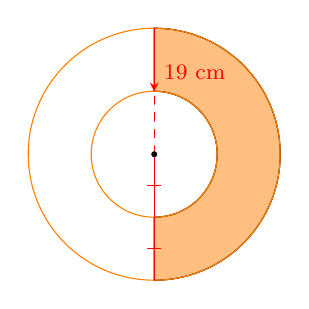
\begin{tikzpicture}[>=stealth,line join=round,line cap=round,font=\footnotesize,scale=0.8]
\def\ra{2}
\def\rb{1}
\path
(0,0) coordinate (O)
(90:\rb) coordinate (M)
(90:\ra) coordinate (N)
(-90:\rb) coordinate (M')
(-90:\ra) coordinate (N')
;
%
\draw[orange] (O)circle(\ra);
\draw[orange] (O)circle(\rb);
\draw[fill=orange!50] (M')--(N')arc (-90:90:\ra)--(N)--(M) arc(90:-90:\rb)--cycle;
\draw[orange] (M')--(N')arc (-90:90:\ra)--(N)--(M) arc(90:-90:\rb)--cycle;
\draw[<-,red](M)--(N) node[pos=0.3,right]{$19$ cm};
\draw[dashed,red](O)--(N);
\draw[red] (O) edge node[midway, sloped, rotate=90, anchor=center] {$ - $}(M');
\draw[red] (M')edge node[midway, sloped, rotate=90, anchor=center] {$ - $}(N');
%	\draw[<->,red] (O)--(M); %\draw[green!50] (O)--(M) node[pos=0.5,above]{$\tiny{ 2\, \text{cm}}$};
%	;
%	\draw[orange!50] (O)--(N);
%	\node at ($(O)+(20:0.6)$){\tiny $72^{\circ}$};
\foreach \x/\y in {O/90}
\draw[fill=black] (\x) circle (1.1pt) + (\y:0.5cm);
%	\draw pic[draw, angle radius=2mm, angle eccentricity=1.5]{right angle = C--A--B};

\end{tikzpicture}\\
Hình $1$& Hình $2$& Hình $3$& Hình $4$\\
\end{tabular}
\end{center}

\loigiai{
\begin{itemize}
\item  Xét hình $1$.\\
$S=\dfrac{\pi\cdot 2^2\cdot 40}{360}=\dfrac{4\pi}{9}$ (cm$^2$).
\item Xét hình $2$.\\
Phần được tô màu có số đo cung là $360^\circ - 72^\circ = 288^\circ$.\\
$S=\dfrac{\pi\cdot 2^2\cdot 288}{360}=\dfrac{16\pi}{5}$ (cm$^2$).
\item Xét hình $3$.\\
$S= \dfrac{1}{4} \pi\left(24^2-6^2\right)=135\pi$ (cm$^2$).
\item Xét hình $4$.\\
$S= \dfrac{\dfrac{1}{4} \pi\left(38^2-19^2\right)}{2}=\dfrac{1083\pi}{8}$ (cm$^2$).
\end{itemize}
}
\end{bt}

\begin{bt}%[Dự án EX-9-Đề Cương Toán 9]%[Phạm Hoàng Điệp]%[9H5H4]
Cho đường tròn $\left(O;R\right)$ và dây $AB$ khác đường kính. Tính khoảng cách từ điểm $O$ đến đường thẳng $AB$, biết $R=5$ cm, $AB=8$ cm.
\loigiai{
\immini{

Gọi $M$ là trung điểm của $AB$ khi đó $OM$ vuông góc $AB$ nên khoảng cách từ điểm $O$ đến đường thẳng $AB$ chính là đoạn thẳng $OM$.\\
$M$ là trung điểm của $AB$ nên $AM=\dfrac{AB}{2}=\dfrac{8}{2}=4$ cm.\\
Xét tam giác $OAM$ vuông tại $M$, có $OA^2=AM^2+OM^2$ (Pythagoras).\\
Suy ra $OM=\sqrt{OA^2-AM^2}=\sqrt{5^2-4^2}=3$ cm.
}
{\begin{tikzpicture}[scale=0.9,font=\footnotesize,line join=round,line cap=round,>=stealth]
\path
(0,0) coordinate (O)
(-30:2) coordinate (A)
(-150:2) coordinate (B)
($(A)!0.5!(B)$) coordinate (M)
;
\draw[thick] (O) circle (2);
\draw[thick] (A)--(O)--(B)--(A) (O)--(M);
\foreach \x/\g in {A/-45,B/-135,O/90,M/-90}
\fill[black] 	(\x) circle (1pt)
($(\g:3mm)+(\x)$) node {$\x$};
\draw pic[draw,,angle radius=3mm]{right angle=A--M--O};
\end{tikzpicture}}
}
\end{bt}

\begin{bt}%[Dự án EX-9-Đề Cương Toán 9]%[Phạm Hoàng Điệp]%[9H5V4]
\immini{ Trong hình bên, cho hai đường tròn có cùng tâm $O$, các điểm $A$, $B$, $C$, $D$ thẳng hàng và $OH \perp AB$ ($H \in AB$).
\begin{enumerate}
\item Chứng minh rằng $AC=BD$.
\item Biết bán kính đường tròn lớn là $10$ cm, $CD=16$ cm và $AB=8$ cm. Tính bán kính đường tròn nhỏ.
\end{enumerate}
}
{
\begin{tikzpicture}[scale=1,font=\footnotesize,line join=round,line cap=round,>=stealth]
\path (0,0) coordinate[label=above:$O$] (O)
(-30:2) coordinate[label=right:$D$] (D)
(-150:2) coordinate[label=left:$C$] (C)
($(C)!.5!(D)$) coordinate[label=above left:$H$] (H);
\draw[name path=circ1] (O) circle (1.25);
\draw (O) circle (2);
\path[name path=line1] (C)--(D);
\path[name intersections={of=line1 and circ1}]
(intersection-1) coordinate[label=below:$A$] (A)
(intersection-2) coordinate[label=below:$B$] (B)
;
\filldraw (O) circle (1pt);
\draw (C)--(D) (O)--(H);
\pic [draw,angle radius=2mm] {right angle=D--H--O};
\end{tikzpicture}
}
\loigiai{
\begin{center}
\begin{tikzpicture}[scale=1,font=\footnotesize,line join=round,line cap=round,>=stealth]
\path (0,0) coordinate[label=above:$O$] (O)
(-30:2) coordinate[label=right:$D$] (D)
(-150:2) coordinate[label=left:$C$] (C)
($(C)!.5!(D)$) coordinate[label=above left:$H$] (H);
\draw[name path=circ1] (O) circle (1.25);
\draw (O) circle (2);
\path[name path=line1] (C)--(D);
\path[name intersections={of=line1 and circ1}]
(intersection-1) coordinate[label=below:$A$] (A)
(intersection-2) coordinate[label=below:$B$] (B)
;
\filldraw (O) circle (1pt);
\draw (C)--(D) (O)--(H) (A)--(O)--(B) (C)--(O)--(D);
\pic [draw,angle radius=2mm] {right angle=D--H--O};
\end{tikzpicture}
\end{center}
\begin{enumerate}
\item
\begin{itemize}
\item
Ta có $OA=OB \Rightarrow \triangle OAB$ cân tại $O$.\\
Xét $\triangle OAB$ cân tại $O$ có: OH là đường cao (vì $OH \perp AB$).\\
Nên $OH$ đồng thời là đường trung tuyến.\\
$\Rightarrow H$ là trung điểm của $AB$.
\item Ta có $OC=OD \Rightarrow \triangle OCD$ cân tại $O$.\\
Xét $\triangle OCD$ cân tại $O$ có: $OH$ là đường cao (vì $OH \perp CD$).\\
Nên $OH$ đồng thời là đường trung tuyến.\\
$\Rightarrow H$ là trung điểm của $CD$.
\item Ta có $\heva{& HC=HD\ (\text{vì $H$ là trung điểm $CD$})\\ & HA=HB\ (\text{vì $H$ là trung điểm $AB$}).}$\\
$\Rightarrow HC-HA=HD-HB$.\\
$\Rightarrow AC=BD$.
\end{itemize}
\item Ta có $\heva{& HD=\dfrac{CD}{2}=\dfrac{16}{2}=8 \mathrm{~cm}\\ & HB=\dfrac{AB}{2}=\dfrac{8}{2}=4 \mathrm{~cm}.}$\\
Xét $\triangle OHD$ vuông tại $H$, ta có:
\allowdisplaybreaks
\begin{eqnarray*}
OD^2 &=& OH^2+HD^2\ (\text{định lí Pythagore})\\
10^2 &=& OH^2+8^2\\
OH^2 &=& 36\\
OH &=& 6 \mathrm{~cm} \, \text{(do $OH>0$)}.
\end{eqnarray*}
Xét $\triangle OHB$ vuông tại $H$, ta có:
\allowdisplaybreaks
\begin{eqnarray*}
OB^2 &=& OH^2+HB^2\ (\text{định lí Pythagore})\\
OB^2 &=& 6^2+4^2\\
OB^2 &=& 52\\
OB &=& 2\sqrt{13} \mathrm{~cm} \, \text{(do $OB>0$)}.
\end{eqnarray*}
\end{enumerate}
}
\end{bt}



\begin{bt}%[Dự án EX-9-Đề Cương Toán 9]%[Phạm Hoàng Điệp]%[9H5C3]
Ba bộ phận truyền chuyển động của một chiếc xe đạp gồm một giò đĩa (bánh răng gắn với bàn đạp), một chiếc líp (cũng có dạng bánh răng) gắn với bánh xe và bộ xích (hình bên dưới). Biết rằng giò đĩa có bán kính $15$ cm, líp có bán kính $4$ cm và bánh xe có đường kính $65$ cm. Hỏi khi người đi xe đạp một vòng thì xe chạy được quãng đường dài bao nhiêu mét (làm tròn đến hàng phần chục)?
\begin{center}
\begin{tikzpicture}
\tikzset{xedap/.pic={
\shade[shading=radial] (-1.5,-2) rectangle (1.5,-1.6);
\shade[shading=radial] (4.5,-2) rectangle (7.5,-1.6);
\def\Radius{1.5cm}
\foreach \a in {0, 10, ..., 350} {
\draw[red] (0, 0) -- (\a:\Radius);
\draw[black] (0, 0) -- (\a+1.5:\Radius);
\draw[gray] (0, 0) -- (\a+3:\Radius);
\draw[gray!50] (0, 0) -- (\a+4.5:\Radius);
\draw[blue] (0, 0) circle[radius=\Radius];
\draw[line width=4pt] (0, 0) circle[radius=\Radius+0.15cm];
}
\foreach \h in {0, 60, ..., 300} {
\draw[color=black,line width=0.5mm,rotate around={\h:(0,0)}] (0,0) edge[-,bend left=40] (0.2cm,0) edge[-,bend right=40] (0.2cm,0);
}
\draw[line width=1pt] (0,0) circle[radius=0.2cm];
\draw[line width=4pt,rounded corners=1pt,rotate=0] (1.68,0.6)--(1.94,0.54);
\draw[line width=0.3mm,yellow!60!black] (1.8,0) arc (0:150:1.8cm)--(0,0);
\draw[line width=0.5mm,yellow!60!black] (1.8,0) arc (0:160:1.8cm);
\foreach \b in {0, 10, ..., 350} {
\draw[color=red,rotate around={\b:(6,0)}] (6, 0) -- (7.5,0);
\draw[black,rotate around={\b+1.5:(6,0)}] (6, 0) -- (7.5,0);
\draw[gray,rotate around={\b+3:(6,0)}] (6, 0) -- (7.5,0);
\draw[gray!50,rotate around={\b+4.5:(6,0)}] (6, 0) -- (7.5,0);
\draw[blue] (6, 0) circle[radius=\Radius];
\draw[line width=4pt] (6, 0) circle[radius=\Radius+0.15cm];
}
\draw[line width=0.3mm,yellow!60!black] (6,1.8) arc (90:190:1.8cm)--(6,0);
\draw[line width=0.5mm,yellow!60!black] (6,1.8) arc (90:200:1.8cm);
\draw[line width=1pt] (0,0.2cm)--(2.2,0.5cm) (0,-0.2cm)--(2.2,-0.5cm);
\draw[line width=2pt] (2.2,0)--(2.6,-0.6) (2.2,0)--(1.8,0.6);
\draw[line width=1mm,rounded corners=8pt,rotate around={25:(6,0)}] (6,0)--(6,1.3cm)--++(80:2.1cm);
\draw[line width=1mm,rounded corners=8pt,rotate around={27:(6,0)}] (6,0)--(6,1.3cm)--++(80:2.1cm);
\draw[line width=1mm,rounded corners=8pt,rotate around={26:(6,0)}] (6,0)--(6,1.3cm)--++(80:2.1cm)coordinate(a);
\draw[line width=1.5mm] (a)--++(-80:0.15cm)--++(0:0.5cm)--++(180:0.05cm)coordinate(b);
\draw[line width=1.1mm,rounded corners=4pt] (b)--++(-30:0.6cm)coordinate(c)--++(-160:0.4cm) (b)--++(150:0.6cm)coordinate(d)--++(200:0.4cm);
\draw[line width=0.4mm,rounded corners=0pt] (c)--++(-95:0.1cm)--++(-160:0.25cm) (d)--++(-95:0.1cm)--++(200:0.25cm);
\draw[line width=2mm,rotate around={35:(2.2,0)}] (2.2,0)--++(3.7,0)--++(75:0.4cm)--++(155:3.5)coordinate(e)--(2.2,0);
\draw[line width=1mm] (0,0)--(2.2,0) (0,0)--(45:2.5cm) (0,0)--(46.5:2.5) (0,0)--(2:2.2);
\draw[line width=1.2mm] (e)--++(106:0.9cm)--++(-74:0.1cm)coordinate(d);
\foreach \c in {0, 72, ..., 288} {\draw[color=red,line width=1.8mm,rotate around={\c:(2.2,0)}] (2.2,0) edge[-,bend left=30] (2.69,0);}
\draw[line width=2pt] (2.2,0) circle[radius=0.5cm];
\fill (2.2,0) circle[radius=0.1cm];
\draw[line width=4pt,rounded corners=1pt,rotate=0] (2.4,-0.58)--(2.68,-0.56);
\draw[line width=2pt] (2.2,0)--(2.6,-0.6);
\shade[top color=white,bottom color=black,rounded corners=2pt,rotate around={10:(d)}] (d)--++(220:2mm)--++(100:2mm)--++(180:3mm)--++(110:1.5mm)--++(160:2mm)--++(110:3.5mm)coordinate(i)--++(-15:10mm)--++(-5:5mm)--++(-20:3mm)coordinate(j)--++(-50:0.7mm)--++(180:4mm)--++(170:1mm)--++(-175:2mm)--(d);
\shade[top color=gray!50,bottom color=black,rounded corners=2pt,rotate around={10:(d)}] (d)--++(220:2mm)--++(100:2mm)--++(180:3mm)--++(110:1.5mm)--++(160:2mm)--++(110:3.5mm)--++(-50:4.5mm)--++(-3:13mm)--++(-10:2mm)--++(180:4mm)--++(170:1mm)--++(-175:2mm)--(d);
\filldraw[black] (0,0)circle(2pt) (6,0)circle(2pt);
\draw[line width=0.3mm] (0,0)--++(105:2cm)--++(-2:0.7cm)coordinate(g)--+(-10:1.5cm) (g)--(0,0);
\shade[top color=gray!10!white,bottom color=gray] (-0.8cm,1.9cm)--++(-3:1.4cm) arc (-90:90: 0.4mm)--++(174:1.4cm) arc (90:270: 0.65mm);
\shade[top color=gray!20,bottom color=black] (-0.8cm,1.9cm)--++(-3:1.4cm) arc (-90:90: 0.4mm)--++(177:1.4cm) arc (90:270: 0.4mm);
}}
\path (0,0) pic[rotate=0,scale=0.8]{xedap};
\draw [<-,thick](1.7,-0.45)--(2,-1.2) node[below,font=\scriptsize]{Giò đĩa};
\end{tikzpicture}
\end{center}
\loigiai{
Chu vi của giò đĩa là $C=2 \cdot \pi\cdot 15=30 \pi$ (cm).\\
Chu vi của líp là $C=2 \cdot \pi\cdot 4=8 \pi$ cm.\\
Chu vi của bánh xe là $C=\pi\cdot65=65 \pi$ cm.\\
Tỉ số chu vi của giò đĩa và chu vi của líp là $\dfrac{30 \pi}{8 \pi}=\dfrac{15}{4}$.\\
Tỉ số vòng quay của líp và vòng quay của giò đĩa là $\dfrac{15}{4}$.\\
Khi líp quay được $1$ vòng thì bánh xe cũng quay được $1$ vòng tương ứng.\\
Suy ra khi giò đĩa quay $1$ vòng thì bánh xe quay được $\dfrac{15}{4}$ vòng.\\
Khi đó mỗi điểm trên bánh xe di chuyển được quãng đường là \[l=\dfrac{15}{4} \cdot65\pi\approx 765{,}8 \text{ (cm) }=7{,}7\text{ (m)}.\]
Vậy người đi xe đạp giò đĩa $1$ vòng liên tục thì xe đạp di chuyển được quãng đường xấp xỉ $7{,}7$ m.
}
\end{bt}














% In đáp án trắc nghiệm
\Closesolutionfile{ans}
\indapan{6}{ans/ans-9C5-OTC}
